\chapter{树}

\section{二叉树的遍历} %%%%%%%%%%%%%%%%%%%%%%%%%%%%%%
\label{sec:binaryTreeTraversal}

在中序遍历中,一个节点的前驱,是其左子树的最右下角结点,后继,是其右子树的最左下角结点。

在后序遍历中,
\begindot
\item 若结点是根结点,则其后继为空;
\item 若结点是双亲的右子树,或是左子树但双亲无右子树,则其后继为双亲结点;
\item 若结点是双亲的左子树且双亲有右子树,则其后继为右子树按后序遍历的第一个结点
\myenddot


\begin{Codex}[label=binary_tree.cpp]
#include <iostream>
#include <stack>
#include <queue>

/** 结点的数据 */
typedef int tree_node_value_t;
 /*
  *@struct
  *@brief 二叉树结点
  */
typedef struct binary_tree_node_t {
    binary_tree_node_t *left;   /* 左孩子*/
    binary_tree_node_t *right;   /* 右孩子*/
    tree_node_value_t value; /* 结点的数据*/
} binary_tree_node_t;

/**
  * @brief 先序遍历,递归.
  * @param[in] root 根结点
  * @param[in] visit 访问数据元素的函数指针
  * @return 无
  */
void pre_order_r(const binary_tree_node_t *root,
                 int (*visit)(const binary_tree_node_t*)) {
    if (root == NULL) return;

    visit(root);
    pre_order_r(root->left, visit);
    pre_order_r(root->right, visit);
}

/**
  * @brief 中序遍历,递归.
  */
void in_order_r(const binary_tree_node_t *root,
                int (*visit)(const binary_tree_node_t*)) {
    if(root == NULL) return;

    in_order_r(root->left, visit);
    visit(root);
    in_order_r(root->right, visit);
}

/**
  * @brief 后序遍历,递归.
  */
void post_order_r(const binary_tree_node_t *root,
                  int (*visit)(const binary_tree_node_t*)) {
    if(root == NULL) return;

    post_order_r(root->left, visit);
    post_order_r(root->right, visit);
    visit(root);
}

/**
 * @brief 先序遍历,非递归.
 */
void pre_order(const binary_tree_node_t *root,
               int (*visit)(const binary_tree_node_t*)) {
    const binary_tree_node_t *p;
    std::stack<const binary_tree_node_t *> s;

    p = root;

    if(p != NULL) s.push(p);

    while(!s.empty()) {
        p = s.top();
        s.pop();
        visit(p);

        if(p->right != NULL) s.push(p->right);
        if(p->left != NULL) s.push(p->left);
    }
}

/**
 * @brief 中序遍历,非递归.
 */
void in_order(const binary_tree_node_t *root,
              int (*visit)(const binary_tree_node_t*)) {
    const binary_tree_node_t *p;
    std::stack<const binary_tree_node_t *> s;

    p = root;

    while(!s.empty() || p!=NULL) {
        if(p != NULL) {
            s.push(p);
            p = p->left;
        } else {
            p = s.top();
            s.pop();
            visit(p);
            p = p->right;
        }
    }
}

/**
 * @brief 后序遍历,非递归.
 */
void post_order(const binary_tree_node_t *root,
                int (*visit)(const binary_tree_node_t*)) {
    /* p,正在访问的结点,q,刚刚访问过的结点*/
    const binary_tree_node_t *p, *q;
    std::stack<const binary_tree_node_t *> s;

    p = root;

    do {
        while(p != NULL) { /* 往左下走*/
            s.push(p);
            p = p->left;
        }
        q = NULL;
        while(!s.empty()) {
            p = s.top();
            s.pop();
            /* 右孩子不存在或已被访问,访问之*/
            if(p->right == q) {
                visit(p);
                q = p; /* 保存刚访问过的结点*/
            } else {
                /* 当前结点不能访问,需第二次进栈*/
                s.push(p);
                /* 先处理右子树*/
                p = p->right;
                break;
            }
        }
    } while(!s.empty());
}

/**
 * @brief 层次遍历,也即BFS.
 *
 * 跟先序遍历一模一样,唯一的不同是栈换成了队列
 */
void level_order(const binary_tree_node_t *root,
                int (*visit)(const binary_tree_node_t*)) {
    const binary_tree_node_t *p;
    std::queue<const binary_tree_node_t *> q;

    p = root;

    if(p != NULL) q.push(p);

    while(!q.empty()) {
        p = q.front();
        q.pop();
        visit(p);

        /*先左后右或先右后左无所谓*/
        if(p->left != NULL) q.push(p->left);
        if(p->right != NULL) q.push(p->right);
    }
}
\end{Codex}

\section{线索二叉树} %%%%%%%%%%%%%%%%%%%%%%%%%%%%%%
二叉树中存在很多空指针,可以利用这些空指针,指向其前驱或者后继。这种利用起来的空指针称为线索,这种改进后的二叉树称为线索二叉树(threaded binary tree)。

一棵n个结点的二叉树含有n+1个空指针。这是因为,假设叶子节点数为$n_0$,度为1的节点数为$n_1$,度为2的节点数为$n_2$,每个叶子节点有2个空指针,每个度为1的节点有1个空指针,则空指针的总数为$2n_0+n_1$,又有$n_0=n_2+1$(留给读者证明),因此空指针总数为$2n_0+n_1=n_0+n_2+1+n_1=n_0+n_1+n_2+1=n+1$。

在二叉树线索化过程中,通常规定,若无左子树,令lchild指向前驱,若无右子树,令rchild指向后继。还需要增加两个标志域表示当前指针是不是线索,例如ltag=1,表示lchild指向的是前驱,ltag=0,表示lchild指向的是左孩子,rtag类似。

二叉树的线索化,实质上就是遍历一棵树,只是在遍历的过程中,检查当前节点的左右指针是否为空,若为空,将它们改为指向前驱或后继的线索。

以中序线索二叉树为例,指针pre表示前驱,succ表示后继,如图~\ref{fig:threadedBinaryTree}所示。

\begin{center}
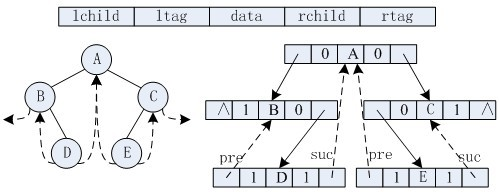
\includegraphics[width=300pt]{threaded-binary-tree.png} \\
\figcaption{中序线索二叉树}\label{fig:threadedBinaryTree}
\end{center}

在中序线索二叉树中,一个节点的前驱,是其左子树的最右下角结点,后继,是其右子树的最左下角结点。

中序线索二叉树的C语言实现如下。
\begin{Codex}[label=theaded_binary_tree.c]
/** @file threaded_binary_tree.c
  * @brief 线索二叉树.
  * @author soulmachine@gmail.com
  * @date 2013-06-16
  */
#include <stddef.h>    /* for NULL */
#include <stdio.h>

/* 结点数据的类型. */
typedef int elem_t;

 /**
  *@struct
  *@brief 线索二叉树结点.
  */
typedef struct tbt_node_t {
    int ltag; /** 1表示是线索,0表示是孩子 */
    int rtag; /** 1表示是线索,0表示是孩子 */
    struct tbt_node_t *lchild; /** 左孩子*/
    struct tbt_node_t *rchild; /** 右孩子*/
    elem_t data; /** 结点所存放的数据*/
}tbt_node_t;

/* 内部函数 */
static void in_thread(tbt_node_t *p, tbt_node_t **pre);
static tbt_node_t *first(tbt_node_t *p);
static tbt_node_t *next(const tbt_node_t *p);

 /**
  * @brief 建立中序线索二叉树.
  * @param[in] root 树根
  * @return 无
  */
void create_in_thread(tbt_node_t *root) {
    /* 前驱结点指针*/
    tbt_node_t *pre=NULL;
    if(root != NULL) { /* 非空二叉树,线索化*/
        /* 中序遍历线索化二叉树*/
        in_thread(root, &pre);
        /* 处理中序最后一个结点*/
        pre->rchild = NULL;
        pre->rtag = 1;
    }
}


/**
  * @brief 在中序线索二叉树上执行中序遍历.
  * @param[in] root 树根
  * @param[in] visit 访问结点的数据的函数
  * @return 无
  */
void in_order(tbt_node_t *root, int(*visit)(elem_t*)) {
    tbt_node_t *p;
    for(p = first(root); p != NULL; p = next(p)) {
        (void)visit(&(p->data));
    }
}


 /*
  * @brief 中序线索化二叉树的主过程.
  * @param[in] p 当前要处理的结点
  * @param[inout] pre 当前结点的前驱结点
  * @return 无
  */
static void in_thread(tbt_node_t *p, tbt_node_t **pre) {
    if(p != NULL) {
        in_thread(p->lchild, pre); /* 线索化左子树 */
        if(p->lchild == NULL) {  /* 左子树为空,建立前驱 */
            p->lchild = *pre;
            p->ltag = 1;
        }
        /* 建立前驱结点的后继线索 */
        if((*pre) != NULL &&
            (*pre)->rchild == NULL) {
            (*pre)->rchild = p;
            (*pre)->rtag = 1;
        }
        *pre = p; /* 更新前驱 */
        in_thread(p->rchild, pre); /* 线索化右子树 */
    }
}

 /*
  * @brief 寻找线索二叉树的中序下的第一个结点.
  * @param[in] p 线索二叉树中的任意一个结点
  * @return 此线索二叉树的第一个结点
  */
static tbt_node_t *first(tbt_node_t *p) {
    if(p == NULL)  return NULL;

    while(p->ltag == 0) {
        p = p->lchild;  /* 最左下结点,不一定是叶结点*/
    }
    return p;
}

 /*
  * @brief 求中序线索二叉树中某结点的后继.
  * @param[in] p 某结点
  * @return p的后继
  */
static tbt_node_t *next(const tbt_node_t *p) {
    if(p->rtag == 0) {
        return first(p->rchild);
    } else {
        return p->rchild;
    }
}
\end{Codex}

中序线索二叉树最简单,在中序线索的基础上稍加修改就可以实现先序,后续就要再费点心思了。


\section{Morris Traversal} %%%%%%%%%%%%%%%%%%%%%%%%%%%%%%
通过前面第\S \ref{sec:binaryTreeTraversal}节,我们知道,实现二叉树的前序(preorder)、中序(inorder)、后序(postorder)遍历有两个常用的方法,一是递归(recursive),二是栈(stack+iterative)。这两种方法都是O(n)的空间复杂度。

而Morris Traversal只需要O(1)的空间复杂度。这种算法跟线索二叉树很像,不过Morris Traversal一边建线索,一边访问数据,访问完后销毁线索,保持二叉树不变。

\subsection{Morris中序遍历}
Morris中序遍历的步骤如下:
\begin{enumerate}
\item 初始化当前节点cur为root节点
\item 如果cur没有左孩子,则输出当前节点并将其右孩子作为当前节点,即cur = cur->rchild。
\item 如果cur有左孩子,则寻找cur的前驱,即cur的左子树的最右下角结点。\\
   a) 如果前驱节点的右孩子为空,将它的右孩子指向当前节点,当前节点更新为当前节点的左孩子。\\
   b) 如果前驱节点的右孩子为当前节点,将它的右孩子重新设为空(恢复树的形状),输出当前节点,当前节点更新为当前节点的右孩子。
\item 重复2、3步骤,直到cur为空。
\end{enumerate}
如图~\ref{fig:inorderMorris}所示,cur表示当前节点,深色节点表示该节点已输出。

\begin{center}
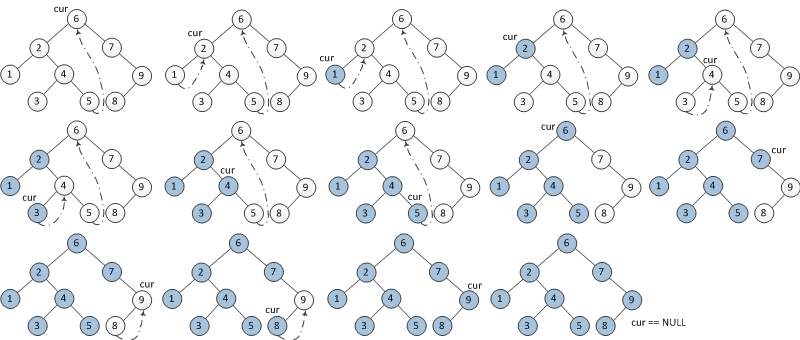
\includegraphics[width=360pt]{inorder-morris-traversal.png} \\
\figcaption{Morris中序遍历}\label{fig:inorderMorris}
\end{center}

C语言实现见第\S\ref{sec:morrisTraversalImpl}节。

\subsubsection{相关的题目}
\begindot
\item Leet Code - Binary Tree Inorder Traversal, \myurl{http://leetcode.com/onlinejudge\#question_94}
\myenddot


\subsection{Morris先序遍历}
Morris先序遍历的步骤如下:
\begin{enumerate}
\item 初始化当前节点cur为root节点
\item 如果cur没有左孩子,则输出当前节点并将其右孩子作为当前节点,即cur = cur->rchild。
\item 如果cur有左孩子,则寻找cur的前驱,即cur的左子树的最右下角结点。\\
   a) 如果前驱节点的右孩子为空,将它的右孩子指向当前节点,\textbf{输出当前节点(在这里输出,这是与中序遍历唯一的不同点)}当前节点更新为当前节点的左孩子。\\
   b) 如果前驱节点的右孩子为当前节点,将它的右孩子重新设为空(恢复树的形状),\sout{输出当前节点,}当前节点更新为当前节点的右孩子。
\item 重复2、3步骤,直到cur为空。
\end{enumerate}
如图~\ref{fig:preorderMorris}所示。

\begin{center}
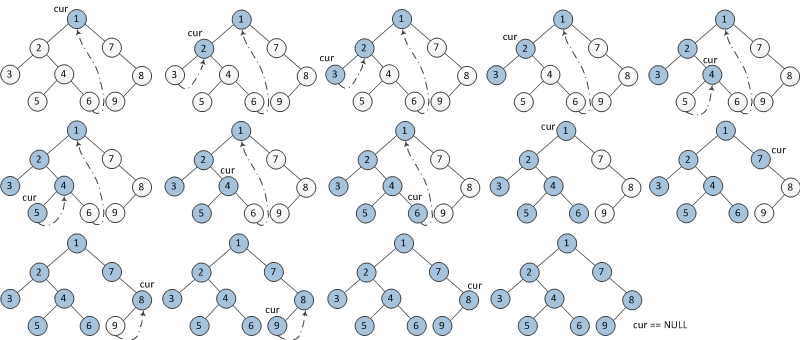
\includegraphics[width=360pt]{preorder-morris-traversal.png} \\
\figcaption{Morris先序遍历}\label{fig:preorderMorris}
\end{center}

C语言实现见第\S\ref{sec:morrisTraversalImpl}节。


\subsection{Morris后序遍历}
Morris后续遍历稍微复杂,需要建立一个临时节点dump,令其左孩子是root,并且还需要一个子过程,就是倒序输出某两个节点之间路径上的所有节点。

Morris后序遍历的步骤如下:
\begin{enumerate}
\item 初始化当前节点cur为root节点
\item 如果cur没有左孩子,则\sout{输出当前节点并}将其右孩子作为当前节点,即cur = cur->rchild。
\item 如果cur有左孩子,则寻找cur的前驱,即cur的左子树的最右下角结点。\\
   a) 如果前驱节点的右孩子为空,将它的右孩子指向当前节点,当前节点更新为当前节点的左孩子。\\
   b) 如果前驱节点的右孩子为当前节点,将它的右孩子重新设为空(恢复树的形状),\sout{输出当前节点,}\textbf{倒序输出从当前节点的左孩子到该前驱节点这条路径上的所有节点。}当前节点更新为当前节点的右孩子。
\item 重复2、3步骤,直到cur为空。
\end{enumerate}
如图~\ref{fig:postorderMorris}所示。

\begin{center}
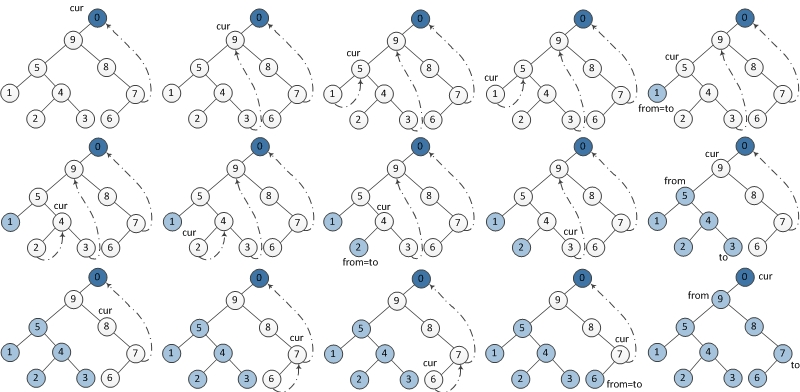
\includegraphics[width=360pt]{postorder-morris-traversal.png} \\
\figcaption{Morris后序遍历}\label{fig:postorderMorris}
\end{center}

C语言实现见第\S\ref{sec:morrisTraversalImpl}节。


\subsection{C语言实现}
\label{sec:morrisTraversalImpl}
\begin{Codex}[label=morris_traversal.cpp]
/** @file morris_traversal.c
 * @brief Morris遍历算法.
 * @author soulmachine@gmail.com
 * @date 2013-06-16
 */
#include<stdio.h>
#include<stdlib.h>

/* 结点数据的类型. */
typedef int elem_t;

/**
 *@struct
 *@brief 二叉树结点.
 */
typedef struct bt_node_t {
    elem_t data; /* 节点的数据 */
    struct bt_node_t *lchild; /* 左孩子 */
    struct bt_node_t *rchild; /* 右孩子 */
} bt_node_t;

/**
 * @brief 中序遍历,Morris算法.
 * @param[in] root 根节点
 * @param[in] visit 访问函数
 * @return 无
 */
void in_order_morris(bt_node_t *root, int(*visit)(elem_t*)) {
    bt_node_t *cur, *prev;

    cur = root;
    while (cur != NULL ) {
        if (cur->lchild == NULL ) {
            visit(cur->data);
            prev = cur;
            cur = cur->rchild;
        } else {
            /* 查找前驱 */
            bt_node_t *node = cur->lchild;
            while (node->rchild != NULL && node->rchild != cur)
                node = node->rchild;

            if (node->rchild == NULL ) { /* 还没线索化,则建立线索 */
                node->rchild = cur;
                prev = cur;
                cur = cur->lchild;
            } else {    /* 已经线索化,则访问节点,并删除线索  */
                visit(cur->data);
                node->rchild = NULL;
                prev = cur;
                cur = cur->rchild;
            }
        }
    }
}

/**
 * @brief 先序遍历,Morris算法.
 * @param[in] root 根节点
 * @param[in] visit 访问函数
 * @return 无
 */
void pre_order_morris(bt_node_t *root, int (*visit)(elem_t*)) {
    bt_node_t *cur, *prev;

    cur = root;
    while (cur != NULL ) {
        if (cur->lchild == NULL ) {
            visit(cur->data);
            prev = cur;
            cur = cur->rchild;
        } else {
            /* 查找前驱 */
            bt_node_t *node = cur->lchild;
            while (node->rchild != NULL && node->rchild != cur)
                node = node->rchild;

            if (node->rchild == NULL ) { /* 还没线索化,则建立线索 */
                visit(cur->data); /* 仅这一行与中序不同 */
                node->rchild = cur;
                prev = cur;
                cur = cur->lchild;
            } else {    /* 已经线索化,则访问节点,并删除线索  */
                node->rchild = NULL;
                prev = cur;
                cur = cur->rchild;
            }
        }
    }
}


static void reverse(bt_node_t *from, bt_node_t *to);
static void visit_reverse(bt_node_t* from, bt_node_t *to, int (*visit)(elem_t*));
/**
 * @brief 后序遍历,Morris算法.
 * @param[in] root 根节点
 * @param[in] visit 访问函数
 * @return 无
 */
void post_order_morris(bt_node_t *root, int (*visit)(elem_t*)) {
    bt_node_t dump = { 0, NULL, NULL };
    dump.lchild = root;
    bt_node_t *cur = &dump, *prev = NULL;
    while (cur != NULL ) {
        if (cur->lchild == NULL ) {
            prev = cur;
            cur = cur->rchild;
        } else {
            bt_node_t *node = cur->lchild;
            while (node->rchild != NULL && node->rchild != cur)
                node = node->rchild;

            if (node->rchild == NULL ) { /* 还没线索化,则建立线索 */
                node->rchild = cur;
                prev = cur;
                cur = cur->lchild;
            } else { /* 已经线索化,则访问节点,并删除线索  */
                visit_reverse(cur->lchild, prev, visit);  // call print
                prev->rchild = NULL;
                prev = cur;
                cur = cur->rchild;
            }
        }
    }
}

/*
 * @brief 逆转路径.
 * @param[in] from from
 * @param[to] to to
 * @return 无
 */
static void reverse(bt_node_t *from, bt_node_t *to) {
    if (from == to) return;
    bt_node_t *x = from, *y = from->rchild, *z;
    while (x != to) {
        z = y->rchild;
        y->rchild = x;
        x = y;
        y = z;
    }
}

/*
 * @brief  访问逆转后的路径上的所有结点.
 * @param[in] from from
 * @param[to] to to
 * @return 无
 */
static void visit_reverse(bt_node_t* from, bt_node_t *to, int (*visit)(elem_t*)) {
    reverse(from, to);

    bt_node_t *p = to;
    while (1) {
        visit(p->data);
        if (p == from)
            break;
        p = p->rchild;
    }

    reverse(to, from);
}

/*
 * @brief 分配一个新节点.
 * @param[in] data 新节点的数据
 * @return 新节点
 */
bt_node_t* new_node(int data) {
    bt_node_t* node = (bt_node_t*) malloc(sizeof(bt_node_t));
    node->data = data;
    node->lchild = NULL;
    node->rchild = NULL;

    return (node);
}

static int print(const elem_t *data) {
    printf(" %d ", data);
    return 0;
}

/* test */
int main() {
    /* 构造的二叉树如下
       1
     /   \
    2      3
  /  \
4     5
     */
    bt_node_t *root = new_node(1);
    root->lchild = new_node(2);
    root->rchild = new_node(3);
    root->lchild->lchild = new_node(4);
    root->lchild->rchild = new_node(5);

    in_order_morris(root, print);
    printf("\n");
    pre_order_morris(root, print);
    printf("\n");
    post_order_morris(root, print);

    return 0;
}
\end{Codex}


\section{重建二叉树} %%%%%%%%%%%%%%%%%%%%%%%%%%%%%%
\begin{Codex}[label=binary_tree_rebuild.c]
#include <stdio.h>
#include <stdlib.h>
#include <string.h>
#include <stddef.h>
/**
 * @brief 给定前序遍历和中序遍历,输出后序遍历.
 *
 * @param[in] pre 前序遍历的序列
 * @param[in] in 中序遍历的序列
 * @param[in] n 序列的长度
 * @param[out] post 后续遍历的序列
 * @return 无
 */
void build_post(const char * pre, const char *in, const int n, char *post) {
    if(n <= 0) return;
    int left_len = strchr(in, pre[0]) - in;
    build_post(pre + 1, in, left_len, post);
    build_post(pre + left_len + 1, in + left_len + 1,
            n - left_len - 1, post + left_len);
    post[n - 1] = pre[0];
}

#define MAX  64
// 测试
// BCAD CBAD,输出 CDAB
// DBACEGF ABCDEFG,输出 ACBFGED
void build_post_test() {
    char pre[MAX] = {0};
    char in[MAX] = {0};
    char post[MAX] = {0};
    scanf("%s%s", pre, in);

    const int n = strlen(pre);
    build_post(pre, in, n, post);
    printf("%s\n", post);
}

/* 结点数据的类型. */
typedef char elem_t;

/**
 *@struct
 *@brief 二叉树结点.
 */
typedef struct bt_node_t {
    elem_t data; /* 节点的数据 */
    struct bt_node_t *lchild; /* 左孩子 */
    struct bt_node_t *rchild; /* 右孩子 */
} bt_node_t;

/**
 * @brief 给定前序遍历和中序遍历,重建二叉树.
 *
 * @param[in] pre 前序遍历的序列
 * @param[in] in 中序遍历的序列
 * @param[in] n 序列的长度
 * @param[out] root 根节点
 * @return 无
 */
void rebuild(const char *pre, const char *in, int n, bt_node_t **root) {
    // 检查终止条件
    if (n <= 0 || pre == NULL || in == NULL)
        return;
    //获得前序遍历的第一个结点
    *root = (bt_node_t*) malloc(sizeof(bt_node_t));
    (*root)->data = *pre;
    (*root)->lchild = NULL;
    (*root)->rchild = NULL;

    int left_len = strchr(in, pre[0]) - in;
    //重建左子树
    rebuild(pre + 1, in, left_len, &((*root)->lchild));
    //重建右子树
    rebuild(pre + left_len + 1, in + left_len + 1, n - left_len - 1,
            &((*root)->rchild));
}

void print_post_order(const bt_node_t *root) {
    if(root != NULL) {
        print_post_order(root->lchild);
        print_post_order(root->rchild);
        printf("%c", root->data);
    }
}

void rebuild_test() {
    char pre[MAX] = { 0 };
    char in[MAX] = { 0 };
    scanf("%s%s", pre, in);
    const int n = strlen(pre);

    bt_node_t *root;
    rebuild(pre, in, n, &root);
    print_post_order(root);
}

int main() {
    build_post_test();
    rebuild_test();
    return 0;
}
\end{Codex}


\section{堆} %%%%%%%%%%%%%%%%%%%%%%%%%%%%%%

\subsection{原理和实现}
C++可以直接使用\fn{std::priority_queue}。

\begin{Codex}[label=heap.c]
/** @file heap.c
 * @brief 堆,默认为小根堆,即堆顶为最小.
 * @author soulmachine@gmail.com
 * @date 2010-8-1
 * @version 1.0
 */
#include <stdlib.h>  /* for malloc() */
#include <string.h>  /* for memcpy() */

typedef int heap_elem_t; // 元素的类型

/**
 * @struct
 * @brief 堆的结构体
 */
typedef struct heap_t {
    int     size;   /** 实际元素个数 */
    int     capacity; /** 容量,以元素为单位 */
    heap_elem_t  *elems;   /** 堆的数组 */
    int (*cmp)(const heap_elem_t*, const heap_elem_t*);   /** 元素的比较函数 */
}heap_t;


/** 基本类型(如int, long, float, double)的比较函数 */
int cmp_int(const int *x, const int *y) {
    const int sub = *x - *y;
    if(sub > 0) {
        return 1;
    } else if(sub < 0) {
        return -1;
    } else {
        return 0;
    }
}

/** 
 * @brief 堆的初始化.
 * @param[out] h 堆对象的指针
 * @param[out] capacity 初始容量
 * @param[in] cmp cmp 比较函数,小于返回-1,等于返回0
 * 大于返回1,反过来则是大根堆
 * @return 成功返回0,失败返回错误码
 */
int heap_init(heap_t *h, const int capacity, 
              int (*cmp)(const heap_elem_t*, const heap_elem_t*)) {
    h->size = 0;
    h->capacity = capacity;
    h->elems = (heap_elem_t*)malloc(capacity * sizeof(heap_elem_t));
    h->cmp = cmp;
    
    return 0;
}

/** 
 * @brief 释放堆.
 * @param[inout] h 堆对象的指针
 * @return 成功返回0,失败返回错误码
 */
int heap_uninit(heap_t *h) {
    h->size = 0;
    h->capacity = 0;
    free(h->elems);
    h->elems = NULL;
    h->cmp = NULL;

    return 0;
}


/** 
 * @brief 判断堆是否为空.
 * @param[in] h 堆对象的指针
 * @return 是空,返回 1,否则返回 0
 */
int heap_empty(const heap_t *h) {
    return h->size == 0;
}

/** 
 * @brief 获取元素个数.
 * @param[in] s 堆对象的指针
 * @return 元素个数
 */
int heap_size(const heap_t *h) {
    return h->size;
}

/*
 * @brief 小根堆的自上向下筛选算法.
 * @param[in] h 堆对象的指针
 * @param[in] start 开始结点
 * @return 无
 */
void heap_sift_down(const heap_t *h, const int start) {
    int i = start;
    int j;
    const heap_elem_t tmp = h->elems[start];
       
    for(j = 2 * i + 1; j < h->size; j = 2 * j + 1) {
        if(j < (h->size - 1) && 
            // h->elems[j] > h->elems[j + 1]
            h->cmp(&(h->elems[j]), &(h->elems[j + 1])) > 0) {
                j++; /* j 指向两子女中小者*/
        }
        // tmp <= h->data[j]
        if(h->cmp(&tmp, &(h->elems[j])) <= 0) {
            break;
        } else {
            h->elems[i] = h->elems[j];
            i = j;
        }
    }
    h->elems[i] = tmp;
}
 
/* 
 * @brief 小根堆的自下向上筛选算法.
 * @param[in] h 堆对象的指针
 * @param[in] start 开始结点
 * @return 无
 */
void heap_sift_up(const heap_t *h, const int start) {
    int j = start;
    int i= (j - 1) / 2;
    const heap_elem_t tmp = h->elems[start];
 
    while(j > 0) {
        // h->data[i] <= tmp
        if(h->cmp(&(h->elems[i]), &tmp) <= 0) {
            break;
        } else {
            h->elems[j] = h->elems[i];
            j = i;
            i = (i - 1) / 2;
        }
    }
    h->elems[j] = tmp;
}

/** 
 * @brief 添加一个元素.
 * @param[in] h 堆对象的指针
 * @param[in] x 要添加的元素
 * @return 无
 */
void heap_push(heap_t *h, const heap_elem_t x) {
    if(h->size == h->capacity) { /*已满,重新分配内存*/
        heap_elem_t* tmp = 
            (heap_elem_t*)realloc(h->elems, h->capacity * 2 * sizeof(heap_elem_t));
        h->elems = tmp;
        h->capacity *= 2;
    }
 
    h->elems[h->size] = x;
    h->size++;

    heap_sift_up(h, h->size - 1);
}

/** 
 * @brief 弹出堆顶元素.
 * @param[in] h 堆对象的指针
 * @return 无
 */
void heap_pop(heap_t *h) {
    h->elems[0] = h->elems[h->size - 1];
    h->size --;
    heap_sift_down(h, 0);
}

/** 
 * @brief 获取堆顶元素.
 * @param[in] h 堆对象的指针
 * @return 堆顶元素
 */
heap_elem_t heap_top(const heap_t *h) {
    return h->elems[0];
}
\end{Codex}


\subsection{最小的N个和} %%%%%%%%%%%%%%%%%%%%%%%%%%%%%%
\subsubsection{描述}
有两个长度为$N$的序列 A 和 B,在 A 和 B 中各任取一个数可以得到 $N^2$ 个和,求这$N^2$ 个和中最小的$N$个。

\subsubsection{输入}
第一行输入一个正整数$N$;第二行N个整数$A_i$ 且$A_i \leq 10^9$;第三行$N$个整数$B_i$,且$Bi \leq 10^9$。

\subsubsection{输出}
输出仅一行,包含$N$个整数,从小到大输出这$N$个最小的和,相邻数字之间用空格隔开。

\subsubsection{样例输入}
\begin{Code}
5
1 3 2 4 5 
6 3 4 1 7
\end{Code}

\subsubsection{样例输出}
\begin{Code}
2 3 4 4 5
\end{Code}

\subsubsection{分析}
由于数据太大,有$N^2$个和,不能通过先求和再排序的方式来求解,这个时候就要用到堆了。

首先将A,B两数组排序,我们可以建立这样一个有序表:
\begin{eqnarray}
A_1+B_1<A_1+B_2<A_1+B_3< &...& <A_1+B_N \nonumber \\
A_2+B_1<A_2+B_2<A_2+B_3< &...& <A_2+B_N \nonumber \\
& ...  \nonumber \\
A_N+B_1<A_N+B_2<A_N+B_3< &...& <A_N+B_N \nonumber
\end{eqnarray}

首先将\fn{A[i] + B[0]}压入堆中,设每次出堆的元素为\fn{sum=A[a]+B[b]},则将\fn{A[a]+B[b+1]}入堆,这样可以保证前$N$个出堆的元素为最小的前$N$项。在实现的时候,可以不用保存B数组的下标,通过\fn{sum-B[b]+B[b+1]}来替换\fn{A[a]+B[b+1]}来节省空间。

\subsubsection{代码}
\begin{Codex}[label=sequence.c]
/* wikioi 1245 最小的N个和,http://www.wikioi.com/problem/1245/  */
#include <stdio.h>
#include <stdlib.h>  /* for malloc() */
#include <string.h>  /* for memcpy() */

#define MAXN 100000

int N;
int a[MAXN], b[MAXN];

typedef struct node_t {
    int sum;
    int b; /* sum=a[i]+b[b] */
} node_t;

typedef node_t heap_elem_t; // 元素的类型
/* 等价于复制粘贴,这里为了节约篇幅,使用include,在OJ上提交时请用复制粘贴 */
#include "heap.c"

void k_merge() {
    heap_t h;
    int i;
    node_t tmp;

    qsort(a, N, sizeof(int), cmp_int);
    qsort(b, N, sizeof(int), cmp_int);
    heap_init(&h, N, cmp_node);

    for (i = 0; i < N; i++) {
        tmp.sum = a[i]+b[0];
        tmp.b = 0;
        heap_push(&h, tmp);
    }

    for (i = 0; i < N; i++) {
        tmp = heap_top(&h); heap_pop(&h);
        printf("%d ", tmp.sum);
        tmp.sum = tmp.sum - b[tmp.b] + b[tmp.b + 1];
        tmp.b++;
        heap_push(&h, tmp);
    }

    heap_uninit(&h);
    return;
}

int main() {
    int i;

    scanf("%d", &N);
    for (i = 0; i < N; i++) {
        scanf("%d", &a[i]);
    }
    for (i = 0; i < N; i++) {
        scanf("%d", &b[i]);
    }

    k_merge();
    return 0;
}
\end{Codex}

\subsubsection{相关的题目}
与本题相同的题目:
\begindot
\item wikioi 1245 最小的N个和, \myurl{http://www.wikioi.com/problem/1245/}
\myenddot

与本题相似的题目:
\begindot
\item  POJ 2442 Sequence, \myurl{http://poj.org/problem?id=2442}
\myenddot


\section{并查集} %%%%%%%%%%%%%%%%%%%%%%%%%%%%%%

\subsection{原理和实现}
通常用树双亲表示作为并查集的存储结构。每个集合以一棵树表示,数组元素的下标代表元素名,根结点的双亲指针为一个负数,表示集合的元素的个数。如图~\ref{fig:ufs1}、图~\ref{fig:ufs2}和图~\ref{fig:ufs3}所示。

\begin{center}
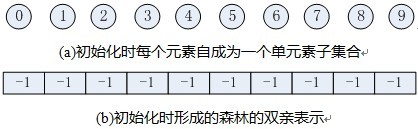
\includegraphics[width=280pt]{ufs1.png}\\
\figcaption{并查集的初始化}\label{fig:ufs1}
\end{center}

\begin{center}
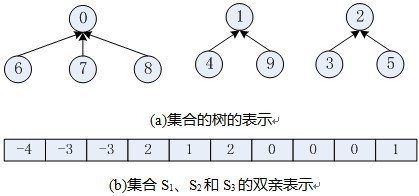
\includegraphics[width=280pt]{ufs2.png}\\
\figcaption{用树表示并查集}\label{fig:ufs2}
\end{center}

\begin{center}
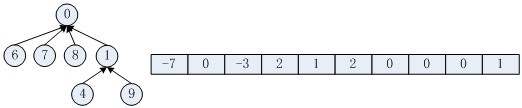
\includegraphics[width=380pt]{ufs3.png}\\
\figcaption{两个集合的并}\label{fig:ufs3}
\end{center}

并查集的C语言实现如下。

\begin{Codex}[label=ufs.c]
#include <stdlib.h>

/** 并查集. */
typedef struct ufs_t {
    int *p;     /** 树的双亲表示法 */
    int size;   /** 大小. */
} ufs_t;

/**
 * @brief 初始化并查集.
 * @param[in] ufs 并查集
 * @param[in] n 数组的容量
 * @return 无
 */
void ufs_init(ufs_t *ufs, int n) {
    int i;
    ufs->p = (int*)malloc(n * sizeof(int));
    for(i = 0; i < n; i++) {
        ufs->p[i] = -1;
    }
}

/**
 * @brief 销毁并查集.
 * @param[in] ufs 并查集
 * @return 无
 */
void ufs_uninit(ufs_t *ufs) {
    free(ufs->p);
    ufs->p = NULL;
    ufs->size = 0;
}

/**
 * @brief Find操作,带路径压缩,递归版.
 * @param[in] s 并查集
 * @param[in] x 要查找的元素
 * @return 包含元素x的树的根
 */
int ufs_find(ufs_t *ufs, int x) {
    if (ufs->p[x] < 0) return x; // 终止条件

    return ufs->p[x] = ufs_find(ufs, ufs->p[x]); /* 回溯时的压缩路径 */
}

/** Find操作,朴素版, deprecated. */
static int ufs_find_naive(ufs_t *ufs, int x) {
    while (ufs->p[x] >= 0) {
        x = ufs->p[x];
    }
    return x;
}

/** Find操作,带路径压缩,迭代版. */
static int ufs_find_iterative(ufs_t *ufs, int x) {
    int oldx = x; /* 记录原始x */
    while (ufs->p[x] >= 0) {
        x = ufs->p[x];
    }
    while (oldx != x) {
        int temp = ufs->p[oldx];
        ufs->p[oldx] = x;
        oldx = temp;
    }
    return x;
}

/**
 * @brief Union操作,将y并入到x所在的集合.
 * @param[in] s 并查集
 * @param[in] x 一个元素
 * @param[in] y 另一个元素
 * @return 如果二者已经在同一集合,并失败,返回-1,否则返回0
 */
int ufs_union(ufs_t *ufs, int x, int y) {
    const int rx = ufs_find(ufs, x);
    const int ry = ufs_find(ufs, y);
    if(rx == ry) return -1;

    ufs->p[rx] += ufs->p[ry];
    ufs->p[ry] = rx;
    return 0;
}

/**
 * @brief 获取元素所在的集合的大小
 * @param[in] ufs 并查集
 * @param[in] x 元素
 * @return 元素所在的集合的大小
 */
int ufs_set_size(ufs_t *ufs, int x) {
    const int rx = ufs_find(ufs, x);
    return -ufs->p[rx];
}
\end{Codex}


\subsection{病毒感染者} %%%%%%%%%%%%%%%%%%%%%%%%%%%%%%
\subsubsection{描述}
一个学校有$n$个社团,一个学生能同时加入不同的社团。由于社团内的同学们交往频繁,如果一个学生感染了病毒,该社团的所有学生都会感染病毒。现在0号学生感染了病毒,问一共有多少个人感染了病毒。

\subsubsection{输入}
输入包含多组测试用例。每个测试用例,第一行包含两个整数$n$,$m$,$n$表示学生个数,$m$表示社团个数。假设$0 < n \leq 30000, 0 \leq m \leq 500$。每个学生从0到$n-1$编号。接下来是$m$行,每行开头是一个整数k,表示该社团的学生个数,接着是$k$个整数表示该社团的学生编号。最后一个测试用例,$n=0,m=0$,表示输入结束。

\subsubsection{输出}
对每个测试用例,输出感染了病毒的学生数目。

\subsubsection{样例输入}
\begin{Code}
100 4
2 1 2
5 10 13 11 12 14
2 0 1
2 99 2
200 2
1 5
5 1 2 3 4 5
1 0
0 0
\end{Code}

\subsubsection{样例输出}
\begin{Code}
4
1
1
\end{Code}

\subsubsection{分析}
非常简单的并查集题目。

\subsubsection{代码}
\begin{Codex}[label=suspects.c]
/* POJ 1611 The Suspects, http://poj.org/problem?id=1611 */
#include <stdio.h>

#define MAXN 30000

/* 等价于复制粘贴,这里为了节约篇幅,使用include,在OJ上提交时请用复制粘贴 */
#include "ufs.c"  /* 见“树->并查集”这节 */

int main() {
    int n, m, k;
    while (scanf("%d%d", &n, &m) && n > 0) {
        ufs_t ufs;
        ufs_init(&ufs, MAXN);
        while (m--) {
            int x, y; /* 两个学生 */
            int rx, ry; /* x, y 所属的集合的根 */
            scanf("%d", &k);

            k--;
            scanf("%d", &x);
            rx = ufs_find(&ufs, x);
            while (k--) {
                scanf("%d", &y);
                ry = ufs_find(&ufs, y);
                ufs_union(&ufs, rx, ry);  /* 只要是跟x同一个集合的都并进去 */
            }
        }
        /* 最后搜索0属于哪个集合,这个集合有多少人 */
        printf("%d\n", ufs_set_size(&ufs, 0));
    }
    return 0;
}
\end{Codex}

\subsubsection{相关的题目}
与本题相同的题目:
\begindot
\item POJ 1611 The Suspects, \myurl{http://poj.org/problem?id=1611}
\myenddot

与本题相似的题目:
\begindot
\item  None
\myenddot


\subsection{两个黑帮} %%%%%%%%%%%%%%%%%%%%%%%%%%%%%%
\subsubsection{描述}
Tadu城市有两个黑帮帮派,已知有$N$黑帮分子,从1到$N$编号,每个人至少属于一个帮派。每个帮派至少有一个人。给你$M$条信息,有两类信息:
\begindot
\item D a b,明确告诉你,a和b属于不同的帮派 
\item A a b,问你,a和b是否属于不同的帮派
\myenddot

\subsubsection{输入}
第一行是一个整数$T$,表示有$T$组测试用例。每组测试用例的第一行是两个整数$N$和$M$,接下来是$M$行,每行包含一条消息。

\subsubsection{输出}
对每条消息"A a b",基于当前获得的信息,输出判断。答案是"In the same gang.", "In different gangs." 和 "Not sure yet."中的一个。

\subsubsection{样例输入}
\begin{Code}
1
5 5
A 1 2
D 1 2
A 1 2
D 2 4
A 1 4
\end{Code}

\subsubsection{样例输出}
\begin{Code}
Not sure yet.
In different gangs.
In the same gang.
\end{Code}

\subsubsection{分析}
把不在一个集合的节点直接用并查集合并在一起。这样的话,如果询问的2个节点在同一个并查集里面,那么它们之间的关系是确定的,否则无法确定它们的关系。

现在还有一个问题是,在同一个集合里面的2个节点是敌对关系还是朋友关系?可以给每个节点另外附加个信息,记录其距离集合根节点的距离。如果,询问的2个节点距离其根节点的距离都是奇数或者都是偶数,那么这2个节点是朋友关系,否则是敌对关系。

\subsubsection{代码}
\begin{Codex}[label=two_gangs.c]
/* POJ 1703 Find them, Catch them, http://poj.org/problem?id=1703 */
#include <stdio.h>
#include <stdlib.h>

#define MAXN 1000001

/** 并查集. */
typedef struct ufs_t {
    int *p;     /** 树的双亲表示法 */
    int *dist;  /** 到根节点的距离的奇偶性 */
    int size;   /** 大小. */
} ufs_t;

/**
 * @brief 初始化并查集.
 * @param[in] ufs 并查集
 * @param[in] n 数组的容量
 * @return 无
 */
void ufs_init(ufs_t *ufs, int n) {
    int i;
    ufs->p = (int*)malloc(n * sizeof(int));
    ufs->dist = (int*)malloc(n * sizeof(int));
    for(i = 0; i < n; i++) {
        ufs->p[i] = -1;
        ufs->dist[i] = 0;
    }
}

/**
 * @brief 销毁并查集.
 * @param[in] ufs 并查集
 * @return 无
 */
void ufs_uninit(ufs_t *ufs) {
    free(ufs->p);
    free(ufs->dist);
    ufs->p = NULL;
    ufs->dist = NULL;
    ufs->size = 0;
}

/**
 * @brief Find操作,带路径压缩,递归版.
 * @param[in] s 并查集
 * @param[in] x 要查找的元素
 * @return 包含元素x的树的根
 */
int ufs_find(ufs_t *ufs, int x) {
    if (ufs->p[x] < 0) return x; // 终止条件

    const int parent = ufs->p[x];
    ufs->p[x] = ufs_find(ufs, ufs->p[x]); /* 回溯时的压缩路径 */
    ufs->dist[x] = (ufs->dist[x] + ufs->dist[parent]) % 2;
    return ufs->p[x];
}

/**
 * @brief Union操作,将root2并入到root1.
 * @param[in] s 并查集
 * @param[in] root1 一棵树的根
 * @param[in] root2 另一棵树的根
 * @return 如果二者已经在同一集合,并失败,返回-1,否则返回0
 */
int ufs_union(ufs_t *ufs, int root1, int root2) {
    if(root1 == root2) return -1;
    ufs->p[root1] += ufs->p[root2];
    ufs->p[root2] = root1;
    return 0;
}

/**
 * @brief 添加一对敌人.
 * @param[inout] s 并查集
 * @param[in] x 一对敌人的一个
 * @param[in] y 一对敌人的另一个
 * @return 无
 */
void ufs_add_opponent(ufs_t *ufs, int x, int y) {
    const int rx = ufs_find(ufs, x);
    const int ry = ufs_find(ufs, y);
    ufs_union(ufs, rx, ry);
    /* ry与y关系 + y与x的关系 + x与rx的关系 = ry与rx的关系 */
    ufs->dist[ry] = (ufs->dist[y] + 1 + ufs->dist[x]) % 2;
}

int main() {
    int T;

    scanf("%d", &T);
    while (T--) {
        ufs_t ufs;
        int n, m;
        char c;
        int x, y, rx, ry;
        scanf("%d%d%*c", &n, &m);
        ufs_init(&ufs, MAXN);

        while (m--) {
            scanf("%c%d%d%*c", &c, &x, &y); //注意输入
            rx = ufs_find(&ufs, x);
            ry = ufs_find(&ufs, y);

            if (c == 'A') {
                if (rx == ry) { //如果根节点相同,则表示能判断关系
                    if (ufs.dist[x] != ufs.dist[y])
                        printf("In different gangs.\n");
                    else
                        printf("In the same gang.\n");
                } else
                    printf("Not sure yet.\n");
            } else if (c == 'D') {
                ufs_add_opponent(&ufs, x, y);
            }
        }
        ufs_uninit(&ufs);
    }
    return 0;
}
\end{Codex}

\subsubsection{相关的题目}
与本题相同的题目:
\begindot
\item POJ 1703 Find them, Catch them, \myurl{http://poj.org/problem?id=1703}
\myenddot

与本题相似的题目:
\begindot
\item  None
\myenddot


\subsection{食物链} %%%%%%%%%%%%%%%%%%%%%%%%%%%%%%
\subsubsection{描述}
动物王国中有三类动物A,B,C,这三类动物的食物链构成了有趣的环形。A吃B, B吃C,C吃A。 现有$N$个动物,从1到$N$编号。每个动物都是A,B,C中的一种,但是我们并不知道它到底是哪一种。 

有人用两种说法对这N个动物所构成的食物链关系进行描述:
\begindot
\item 第一种说法是"1 X Y",表示X和Y是同类。 
\item 第二种说法是"2 X Y",表示X吃Y。 
\myenddot

此人对$N$个动物,用上述两种说法,一句接一句地说出$K$句话,这$K$句话有的是真的,有的是假的。当一句话满足下列三条之一时,这句话就是假话,否则就是真话。 
\begindot
\item 当前的话与前面的某些真的话冲突,就是假话; 
\item 当前的话中X或Y比N大,就是假话; 
\item 当前的话表示X吃X,就是假话。 
\myenddot

你的任务是根据给定的$N(1 \leq N \leq 50,000)$和$K$句话($0 \leq K \leq 100,000$),输出假话的总数。 

\subsubsection{输入}
第一行是两个整数$N$和$K$,以一个空格分隔。 

以下$K$行每行是三个正整数D,X,Y,两数之间用一个空格隔开,其中D表示说法的种类。
\begindot
\item 若D=1,则表示X和Y是同类。 
\item 若D=2,则表示X吃Y。
\myenddot

\subsubsection{输出}
只有一个整数,表示假话的数目。

\subsubsection{样例输入}
\begin{Code}
100 7
1 101 1 
2 1 2
2 2 3 
2 3 3 
1 1 3 
2 3 1 
1 5 5
\end{Code}

\subsubsection{样例输出}
\begin{Code}
3
\end{Code}

\subsubsection{分析}


\subsubsection{代码}
\begin{Codex}[label=food_chain.c]
/* POJ 1182 食物链, Catch them, http://poj.org/problem?id=1182 */
#include <stdio.h>
#include <stdlib.h>

/** 并查集. */
typedef struct ufs_t {
    int *p;     /** 树的双亲表示法 */
    int *dist;  /** 表示x与父节点p[x]的关系,0表示x与p[x]是同类,
                    1表示x吃p[x],2表示p[x]吃x */
    int size;   /** 大小. */
} ufs_t;

/**
 * @brief 初始化并查集.
 * @param[in] ufs 并查集
 * @param[in] n 数组的容量
 * @return 无
 */
void ufs_init(ufs_t *ufs, int n) {
    int i;
    ufs->p = (int*)malloc(n * sizeof(int));
    ufs->dist = (int*)malloc(n * sizeof(int));
    for(i = 0; i < n; i++) {
        ufs->p[i] = -1;
        ufs->dist[i] = 0; // 自己与自己是同类
    }
}

/**
 * @brief 销毁并查集.
 * @param[in] ufs 并查集
 * @return 无
 */
void ufs_uninit(ufs_t *ufs) {
    free(ufs->p);
    free(ufs->dist);
    ufs->p = NULL;
    ufs->dist = NULL;
    ufs->size = 0;
}

/**
 * @brief Find操作,带路径压缩,递归版.
 * @param[in] s 并查集
 * @param[in] x 要查找的元素
 * @return 包含元素x的树的根
 */
int ufs_find(ufs_t *ufs, int x) {
    if (ufs->p[x] < 0) return x; // 终止条件

    const int parent = ufs->p[x];
    ufs->p[x] = ufs_find(ufs, ufs->p[x]); /* 回溯时的压缩路径 */
    /* 更新关系 */
    ufs->dist[x] = (ufs->dist[x] + ufs->dist[parent]) % 3;
    return ufs->p[x];
}

/**
 * @brief Union操作,将root2并入到root1.
 * @param[in] s 并查集
 * @param[in] root1 一棵树的根
 * @param[in] root2 另一棵树的根
 * @return 如果二者已经在同一集合,并失败,返回-1,否则返回0
 */
int ufs_union(ufs_t *ufs, int root1, int root2) {
    if(root1 == root2) return -1;
    ufs->p[root1] += ufs->p[root2];
    ufs->p[root2] = root1;
    return 0;
}

/**
 * @brief 添加一对关系.
 * @param[inout] s 并查集
 * @param[in] x 一个
 * @param[in] y 另一个
 * @param[in] len
 * @return 无
 */
void ufs_add_relation(ufs_t *ufs, int x, int y, int relation) {
    const int rx = ufs_find(ufs, x);
    const int ry = ufs_find(ufs, y);
    ufs_union(ufs, ry, rx); /* 注意顺序! */
    /* rx与x关系 + x与y的关系 + y与ry的关系 = rx与ry的关系 */
    ufs->dist[rx] = (ufs->dist[y] - ufs->dist[x] + 3 + relation) % 3;
}

int main() {
    int n, k;
    int result = 0; /* 假话的数目 */
    ufs_t ufs;

    scanf("%d%d", &n, &k);
    ufs_init(&ufs, n+1);

    while(k--) {
        int d, x, y;
        scanf("%d%d%d", &d, &x, &y);

        if (x > n || y > n || (d == 2 && x == y)) {
            result++;
        } else {
            const int rx = ufs_find(&ufs, x);
            const int ry = ufs_find(&ufs, y);

            if (rx == ry) { /* 若在同一个集合则可确定x和y的关系 */
                if((ufs.dist[x] - ufs.dist[y] + 3) % 3 != d - 1)
                    result++;
            } else {
                ufs_add_relation(&ufs, x, y, d-1);
            }
        }
    }

    printf("%d\n", result);

    ufs_uninit(&ufs);
    return 0;
}
\end{Codex}

\subsubsection{相关的题目}
与本题相同的题目:
\begindot
\item POJ 1182 食物链, \myurl{http://poj.org/problem?id=1182}
\item wikioi 1074 食物链, \myurl{http://www.wikioi.com/problem/1074/}
\myenddot

与本题相似的题目:
\begindot
\item  None
\myenddot


\section{线段树} %%%%%%%%%%%%%%%%%%%%%%%%%%%%%%

\subsection{原理和实现}
\textbf{线段树},也叫区间树(interval tree),它在各个节点保存一条线段(即子数组)。设数列$A$包含$N$个元素,则线段树的根节点表示整个区间$A[1,N]$,左孩子表示区间$A[1, (1+N)/2]$,右孩子表示区间$A[(1+N)/2+1, N]$,不断递归,直到叶子节点,叶子节点只包含一个元素。

线段树有如下特征:
\begindot
\item 线段树是一棵完全二叉树
\item 线段树的深度不超过$\log L$, $L$是区间的长度
\item 线段树把一个长度为L的区间分成不超过$2\log L$条线段
\myenddot

线段树的基本操作有构造线段树、区间查询和区间修改。

线段树通常用于解决和区间统计有关的问题。比如某些数据可以按区间进行划分,按区间动态进行修改,而且还需要按区间多次进行查询,那么使用线段树可以达到较快的查询速度。

用线段树解题,关键是要想清楚每个节点要存哪些信息(当然区间起点和终点,以及左右孩子指针是必须的),以及这些信息如何高效查询,更新。不要一更新就更新到叶子节点,那样更新操作的效率最坏有可能$O(N)$的。

\subsection{Balanced Lineup} %%%%%%%%%%%%%%%%%%%%%%%%%%%%%%
\subsubsection{描述}
给定$N(1 \leq N \leq 50,000)$ 个数, $A_1, A_2, ... , A_N$,求任意区间中最大数和最小数的差。

\subsubsection{输入}
第一行包含两个整数,$N$和$Q$。$Q$表示查询次数。

第2到N+1行,每行包含一个整数$A_i$。

第N+2到N+Q+1行,每行包含两个整数$a$和$b(1 \leq a \leq b \leq N)$,表示区间$A[a,b]$。

\subsubsection{输出}
对每个查询进行回应,输出该区间内最大数和最小数的差

\subsubsection{样例输入}
\begin{Code}
6 3
1
7
3
4
2
5
1 5
4 6
2 2
\end{Code}

\subsubsection{样例输出}
\begin{Code}
6
3
0
\end{Code}

\subsubsection{分析}
本题是“区间求和”,只需要“线段树构造”和“区间查询”两个操作。

\subsubsection{代码}
\begin{Codex}[label=balanced_lineup.c]
#include <stdio.h>
#include <stdlib.h>
#include <string.h>
#include <limits.h>

#define MAXN 50001
#define INF INT_MAX
#define max(a,b) ((a)>(b)?(a):(b))
#define min(a,b) ((a)<(b)?(a):(b))
#define L(a) ((a)<<1)
#define R(a) (((a)<<1)+1)

typedef struct node_t {
    int left, right;  /* 区间  */
    int max, min;  /* 本区间里的最大值和最小值 */
} node_t;

int A[MAXN]; /* 输入数据,0位置未用 */

/* 完全二叉树,结点编号从1开始,层次从1开始.
 * 用一维数组存储完全二叉树,空间约为4N,
 * 参考 http://comzyh.tk/blog/archives/479/
 */
node_t node[MAXN * 4];

int minx, maxx; /* 存放查询的结果 */

void init() {
    memset(node, 0, sizeof(node));
}

/* 以t为根结点,为区间A[l,r]建立线段树 */
void build(int t, int l, int r) {
    node[t].left = l, node[t].right = r;
    if (l == r) {
        node[t].max = node[t].min = A[l];
        return;
    }
    const int mid = (l + r) / 2;
    build(L(t), l, mid);
    build(R(t), mid + 1, r);
    node[t].max = max(node[L(t)].max,node[R(t)].max);
    node[t].min = min(node[L(t)].min,node[R(t)].min);
}

/* 查询根结点为t,区间为A[l,r]的最大值和最小值 */
void query(int t, int l, int r) {
    if (node[t].left == l && node[t].right == r) {
        if (maxx < node[t].max)
            maxx = node[t].max;
        if (minx > node[t].min)
            minx = node[t].min;
        return;
    }
    const int mid = (node[t].left + node[t].right) / 2;
    if (l > mid) {
        query(R(t), l, r);
    } else if (r <= mid) {
        query(L(t), l, r);
    } else {
        query(L(t), l, mid);
        query(R(t), mid + 1, r);
    }
}

int main() {
    int n, q, i;

    scanf("%d%d", &n, &q);
    for (i = 1; i <= n; i++) scanf("%d", &A[i]);

    init();
    /* 建立以tree[1]为根结点,区间为A[1,n]的线段树 */
    build(1, 1, n);

    while (q--) {
        int a, b;
        scanf("%d%d", &a, &b);
        maxx = 0;
        minx = INF;
        query(1, a, b); /* 查询区间A[a,b]的最大值和最小值 */
        printf("%d\n", maxx - minx);
    }
    return 0;
}
\end{Codex}

\subsubsection{相关的题目}
与本题相同的题目:
\begindot
\item POJ 3264 Balanced Lineup, \myurl{http://poj.org/problem?id=3264}
\myenddot

与本题相似的题目:
\begindot
\item  None
\myenddot


\subsection{线段树练习 1} %%%%%%%%%%%%%%%%%%%%%%%%%%%%%%
\subsubsection{描述}
一行$N(1\leq N < 100000)$个方格,开始每个格子里都有一个整数。现在动态地提出一些命令请求,有两种命令,查询和增加:求某一个特定的子区间$[a,b]$中所有元素的和;指定某一个格子$x$,加上一个特定的值A。现在要求你能对每个请求作出正确的回答。

\subsubsection{输入}
输入文件第一行为一个整数$N$,接下来是$n$行每行1个整数,表示格子中原来的整数。接下来是一个正整数$Q$,再接下来有$Q$行,表示$Q$个询问,第一个整数表示命令代号,命令代号1表示增加,后面的两个数$a$和$x$表示给位置$a$上的数值增加$x$,命令代号2表示区间求和,后面两个整数a和b,表示要求[a,b]之间的区间和。

\subsubsection{输出}
共$Q$行,每个整数

\subsubsection{样例输入}
\begin{Code}
6
4 
5 
6 
2 
1 
3
4
1 3 5
2 1 4
1 1 9
2 2 6
\end{Code}

\subsubsection{样例输出}
\begin{Code}
22
22
\end{Code}

\subsubsection{分析}
单点更新+区间求和

\subsubsection{代码}
\begin{Codex}[label=interval_tree1.c]
/* wikioi 1080 线段树练习 , http://www.wikioi.com/problem/1080/ */
#include <stdio.h>
#include <string.h>

#define L(a) ((a)<<1)
#define R(a) (((a)<<1)+1)
#define MAXN 100001

typedef long long int64_t;

typedef struct node_t {
    int left, right;
    int64_t sum;
} node_t;

int A[MAXN]; /* 输入数据,0位置未用 */

/* 完全二叉树,结点编号从1开始,层次从1开始.
 * 用一维数组存储完全二叉树,空间约为4N,
 * 参考 http://comzyh.tk/blog/archives/479/
 */
node_t node[MAXN * 4];

void init() {
    memset(node, 0, sizeof(node));
}

/* 以t为根结点,为区间A[l,r]建立线段树 */
void build(int t, int l, int r) {
    node[t].left = l;
    node[t].right = r;
    if (l == r) {
        node[t].sum = A[l];
        return;
    }
    const int mid = (l + r) / 2;
    build(L(t), l, mid);
    build(R(t), mid + 1, r);
    node[t].sum = node[L(t)].sum + node[R(t)].sum;
}

/* 给区间A[l,r]里的pos位置加delta */
void update(int t, int l, int r, int pos, int64_t delta) {
    if (node[t].left > pos || node[t].right < pos) return;
    if (node[t].left == node[t].right) {
        node[t].sum += delta;
        return;
    }

    const int mid = (node[t].left + node[t].right) / 2;
    if (l > mid) update(R(t), l, r, pos, delta);
    else if (r <= mid) update(L(t), l, r, pos, delta);
    else {
        update(L(t), l, mid, pos, delta);
        update(R(t), mid + 1, r, pos, delta);
    }
    node[t].sum = node[L(t)].sum + node[R(t)].sum;
}

/* 查询根结点为t,区间为A[l,r]的和 */
int64_t query(int t, int l, int r) {
    if (node[t].left == l && node[t].right == r)
        return node[t].sum;
    const int mid = (node[t].left + node[t].right) / 2;
    if (l > mid) return query(R(t), l, r);
    else if (r <= mid) return query(L(t), l, r);
    else return query(L(t), l, mid) + query(R(t), mid + 1, r);
}

int main() {
    int i, n, q;
    scanf("%d", &n);
    for (i = 1; i <= n; i++) scanf("%d", &A[i]);

    init();
    /* 建立以tree[1]为根结点,区间为A[1,n]的线段树 */
    build(1, 1, n);

    scanf("%d", &q);
    while (q--) {
        int cmd;
        scanf("%d", &cmd);
        if (cmd == 2) {
            int a, b;
            scanf("%d%d", &a, &b);
            printf("%lld\n", query(1, a, b)); /* 查询区间A[a,b]的和 */
        } else {
            int a;
            int64_t x;
            scanf("%d%lld", &a, &x);
            if (x != 0) update(1, 1, n, a, x);
        }
    }
    return 0;
}
\end{Codex}

\subsubsection{相关的题目}
与本题相同的题目:
\begindot
\item wikioi 1080 线段树练习 1, \myurl{http://www.wikioi.com/problem/1080/}
\myenddot

与本题相似的题目:
\begindot
\item  wikioi 1081 线段树练习 2, \myurl{http://www.wikioi.com/problem/1081/} 。本题是“区间更新+单点查询”,可以转化为线段树练习1。设原数组为$A[N]$,将其转化为差分数列,然后在数组上维护一棵线段树。“区间更新”操作转化为两个“单点更新”操作:将$A[a]$加上$x$,并将$A[b+1]$减去$x$(也就是加上$-x$)。“单点查询”操作转化为“区间求和”操作:求$A$数组$[1..i]$范围内所有数的和。这样就转化成与线段树练习1完全相同了。标程 \myurl{https://gist.github.com/soulmachine/6449609}
\myenddot


\subsection{A Simple Problem with Integers} %%%%%%%%%%%%%%%%%%%%%%%%%%%%%%
\subsubsection{描述}
You have $N$ integers, $A_1, A_2, ... , A_N$. You need to deal with two kinds of operations. One type of operation is to add some given number to each number in a given interval. The other is to ask for the sum of numbers in a given interval.

\subsubsection{输入}
The first line contains two numbers $N$ and $Q$. $1 \leq N,Q \leq 100000$.

The second line contains $N$ numbers, the initial values of $A_1, A_2, ... , A_N$. $-1000000000 \leq A_i \leq 1000000000$.

Each of the next $Q$ lines represents an operation.
"C a b c" means adding $c$ to each of $A_a, A_{a+1}, ... , A_b$. $-10000 ≤ c ≤ 10000$.
"Q a b" means querying the sum of $A_a, A_{a+1}, ... , A_b$.

\subsubsection{输出}
You need to answer all $Q$ commands in order. One answer in a line.

\subsubsection{样例输入}
\begin{Code}
10 5
1 2 3 4 5 6 7 8 9 10
Q 4 4
Q 1 10
Q 2 4
C 3 6 3
Q 2 4
\end{Code}

\subsubsection{样例输出}
\begin{Code}
4
55
9
15
\end{Code}

\subsubsection{提示}
The sums may exceed the range of 32-bit integers.

\subsubsection{分析}
区间更新+区间求和。

树节点要存哪些信息?只存该区间的和,行不行?只存和,会导致每次加数的时候都要更新到叶子节点,速度太慢。本题节点的结构如下:
\begin{Code}
typedef struct node_t {
    int left, right;
    int64_t sum;  /* 本区间的和实际上是sum+inc*[right-left+1] */
    int64_t inc;  /* 增量c的累加 */
} node_t;
\end{Code}

\subsubsection{代码}
\begin{Codex}[label=poj3468.c]
#include <stdio.h>
#include <string.h>

#define L(a) ((a)<<1)
#define R(a) (((a)<<1)+1)
#define MAXN 100001

typedef long long int64_t;

typedef struct node_t {
    int left, right;
    int64_t sum;  /* 本区间的和实际上是sum+inc*[right-left+1] */
    int64_t inc;  /* 增量c的累加 */
} node_t;

int A[MAXN]; /* 输入数据,0位置未用 */

/* 完全二叉树,结点编号从1开始,层次从1开始.
 * 用一维数组存储完全二叉树,空间约为4N,
 * 参考 http://comzyh.tk/blog/archives/479/
 */
node_t node[MAXN * 4];

void init() {
    memset(node, 0, sizeof(node));
}

/* 以t为根结点,为区间A[l,r]建立线段树 */
void build(int t, int l, int r) {
    node[t].left = l;
    node[t].right = r;
    if (l == r) {
        node[t].sum = A[l];
        return;
    }
    const int mid = (l + r) / 2;
    build(L(t), l, mid);
    build(R(t), mid+1, r);
    node[t].sum = node[L(t)].sum + node[R(t)].sum;
}

/* 给区间A[l,r]里的每个元素都加c */
void update(int t, int l, int r, int64_t c) {
    if (node[t].left == l && node[t].right == r) {
        node[t].inc += c;
        node[t].sum += c * (r - l + 1);
        return;
    }
    if (node[t].inc) {
        node[R(t)].inc += node[t].inc;
        node[L(t)].inc += node[t].inc;
        node[R(t)].sum += node[t].inc * (node[R(t)].right - node[R(t)].left + 1);
        node[L(t)].sum += node[t].inc * (node[L(t)].right - node[L(t)].left + 1);
        node[t].inc = 0;
    }
    const int mid = (node[t].left + node[t].right) / 2;
    if (l > mid)
        update(R(t), l, r, c);
    else if (r <= mid)
        update(L(t), l, r, c);
    else {
        update(L(t), l, mid, c);
        update(R(t), mid + 1, r, c);
    }
    node[t].sum = node[L(t)].sum + node[R(t)].sum;
}

/* 查询根结点为t,区间为A[l,r]的和 */
int64_t query(int t, int l, int r) {
    if (node[t].left == l && node[t].right == r)
        return node[t].sum;
    if (node[t].inc) {
        node[R(t)].inc += node[t].inc;
        node[L(t)].inc += node[t].inc;
        node[R(t)].sum += node[t].inc * (node[R(t)].right - node[R(t)].left + 1);
        node[L(t)].sum += node[t].inc * (node[L(t)].right - node[L(t)].left + 1);
        node[t].inc = 0;
    }
    const int mid = (node[t].left + node[t].right) / 2;
    if (l > mid)
        return query(R(t), l, r);
    else if (r <= mid)
        return query(L(t), l, r);
    else
        return query(L(t), l, mid) + query(R(t), mid + 1, r);
}

int main() {
    int i, n, q;
    char s[5];
    scanf("%d%d", &n, &q);
    for (i = 1; i <= n; i++) scanf("%d", &A[i]);

    init();
    /* 建立以tree[1]为根结点,区间为A[1,n]的线段树 */
    build(1, 1, n);

    while (q--) {
        int a, b;
        int64_t c;
        scanf("%s", s);
        if (s[0] == 'Q') {
            scanf("%d%d", &a, &b);
            printf("%lld\n", query(1, a, b)); /* 查询区间A[a,b]的和 */
        } else {
            scanf("%d%d%lld", &a, &b, &c);
            if (c != 0) update(1, a, b, c);
        }
    }
    return 0;
}
\end{Codex}

\subsubsection{相关的题目}
与本题相同的题目:
\begindot
\item POJ 3468 A Simple Problem with Integers, \myurl{http://poj.org/problem?id=3468}
\myenddot

与本题相似的题目:
\begindot
\item None
\myenddot


\subsection{约瑟夫问题} %%%%%%%%%%%%%%%%%%%%%%%%%%%%%%
\subsubsection{描述}
有编号从1到$N$的$N$个小朋友在玩一种出圈的游戏。开始时$N$个小朋友围成一圈,编号为$i+1$的小朋友站在编号为$i$小朋友左边。编号为1的小朋友站在编号为$N$的小朋友左边。首先编号为1的小朋友开始报数,接着站在左边的小朋友顺序报数,直到数到某个数字$M$时就出圈。直到只剩下1个小朋友,则游戏完毕。

现在给定$N,M$,求$N$个小朋友的出圈顺序。

\subsubsection{输入}
唯一的一行包含两个整数$N,M(1 \leq N,M \leq 30000)$。

\subsubsection{输出}
唯一的一行包含$N$个整数,每两个整数中间用空格隔开,第$i$个整数表示第$i$个出圈的小朋友的编号。

\subsubsection{样例输入}
\begin{Code}
5 3
\end{Code}

\subsubsection{样例输出}
\begin{Code}
3 1 5 2 4
\end{Code}

\subsubsection{分析}
约瑟夫问题的难点在于,每一轮都不能通过简单的运算得出下一轮谁淘汰,因为中间有人已经退出了。因此一般只能模拟,效率很低。

现在考虑,每一轮都令所有剩下的人从左到右重新编号,例如3退出后,场上还剩下1、2、4、5,则给1新编号1,2新编号2,4新编号3,5新编号4。不妨称这个编号为“剩余队列编号”。如下所示,括号内为原始编号:
\begin{Code}
1(1) 2(2) 3(3) 4(4) 5(5) --> 剩余队列编号3淘汰,对应原编号3
1(1) 2(2) 3(4) 4(5) --> 剩余队列编号1淘汰,对应原编号1
1(2) 2(4) 3(5) --> 剩余队列编号3淘汰,对应原编号5
1(2) 2(4) --> 剩余队列编号1淘汰,对应原编号2
1(4) --> 剩余队列编号1滔天,对应原编号4
\end{Code}

一个人在当前剩余队列中编号为$i$,则说明他是从左到右数第$i$个人,这启发我们可以用线段树来解决问题。用线段树维护原编号$[i..j]$内还有多少人没 有被淘汰,这样每次选出被淘汰者后,在当前线段树中查找位置就可以了。

例如我们有5个原编号,当前淘汰者在剩余队列中编号为3,先看左子树,即原编号[1..3]区间内,如果剩下的人不足3个,则说明当前剩余编号为3的 这个人原编号只能是在[4..5]区间内,继续在[4..5]上搜索;如果[1..3]内剩下的人大于等于3个,则说明就在[1..3]内,也继续缩小范围查找,这样即可在$O(\log N)$时间内完成对应。问题得到圆满的解决。

\subsubsection{代码}
\begin{Codex}[label=josephus_problem.c]
/* wikioi 1282 约瑟夫问题, http://www.wikioi.com/problem/1282/ */
#include <stdio.h>
#include <string.h>

#define L(a) ((a)<<1)
#define R(a) (((a)<<1)+1)
#define MAXN 30001

typedef struct node_t {
    int left, right;
    int count; /* 区间内的元素个数 */
} node_t;

/* 完全二叉树,结点编号从1开始,层次从1开始.
 * 用一维数组存储完全二叉树,空间约为4N,
 * 参考 http://comzyh.tk/blog/archives/479/
 */
node_t node[MAXN * 4];

void init() {
    memset(node, 0, sizeof(node));
}

/* 以t为根结点,为区间[l,r]建立线段树 */
void build(int t, int l, int r) {
    node[t].left = l;
    node[t].right = r;
    node[t].count = r - l + 1;
    if (l == r) return;

    const int mid = (r + l) / 2;
    build(L(t), l, mid);
    build(R(t), mid + 1, r);
}

/**
 * @brief 输出i
 * @param[in] t 根节点
 * @param[in] i 剩余队列编号
 * @return 被删除的实际数字
 */
int delete(int t, int i) {
    node[t].count--;
    if (node[t].left == node[t].right) {
        printf("%d ", node[t].left);
        return node[t].left;
    }
    if (node[L(t)].count >= i) return delete(L(t), i);
    else return delete(R(t), i - node[L(t)].count); /* 左子树人数不足,则在右子树查找 */
}

/**
 * @brief 返回 1到i内的活人数
 * @param[in] t 根节点
 * @param[in] i 原始队列的数字
 * @return 1到i内的活人数
 */
int get_count(int t, int i) {
    if (node[t].right <= i) return node[t].count;

    const int mid = (node[t].left + node[t].right) / 2;
    int s = 0;
    if (i > mid) {
        s += node[L(t)].count;
        s += get_count(R(t), i);
    } else
        s += get_count(L(t), i);
    return s;
}

int main() {
    int n, m;
    scanf("%d%d", &n, &m);

    init();
    build(1, 1, n);

    int i;
    int j = 0; /* 剩余队列的虚拟编号 */
    for (i = 1; i <= n; i++) {
        j += m;
        if (j > node[1].count)
            j %= node[1].count;
        if (j == 0) j = node[1].count;
        const int k = delete(1, j);
        j = get_count(1, k);
    }
    return 0;
}
\end{Codex}

\subsubsection{相关的题目}
与本题相同的题目:
\begindot
\item wikioi 1282 约瑟夫问题, \myurl{http://www.wikioi.com/problem/1282/}
\myenddot

与本题相似的题目:
\begindot
\item None
\myenddot
